\section{Introduction}
\label{sec:introduction}

A letter of intent \cite{Bonivento:2013jag} for a new experiment at CERN intended to search for hidden particles with the use of intensive beam of protons of SPS accelerator was submitted to SPSC  in 2013.  The SHiP collaboration that has been formed as a result prepared in 2015 two documents describing the physics case \cite{Alekhin:2015byh},  and a technical proposal \cite{Anelli:2015pba} of SHiP. The present paper provides an update of  the physics case and describes developments and advances in the technical design of the proposed experiment.

\section{Overview of changes since Technical Proposal}

\subsection{Physics Landscape}

{\bf Physics landscape in 2015.}  The discovery of the Higgs boson at the LHC in 2012 \cite{ATLAS:2012ae,Aad:2012tfa,Chatrchyan:2012tx,Chatrchyan:2012ufa}  made the Standard Model (SM) of elementary particles complete - all the particles predicted by it have been found, and their interactions,  tested at the LHC till now,  are consistent with those predicted by the SM. The triumph of the SM in particle physics is accompanied by the success  of the standard cosmological model based on Einstein's General Relativity -- $\Lambda$CDM, allowing to describe the structure of the Universe by a small number of parameters.

The quest for the new particles has not ended, however. Indeed we are certain that the SM is not complete. Several well-established observational phenomena -- neutrino masses and oscillations, dark matter, and baryon asymmetry of the Universe -- cannot be explained with known particles alone and clearly indicate that more particles should exist. Unfortunately, we do not have a definite prediction where to find this New Physics (NP), what masses, spins, and coupling constants these new particles should have. The era of guaranteed discoveries in particle physics has finished  with the detecting of the Higgs boson: for the particular value of the Higgs mass revealed by the LHC, the Standard Model remains mathematically consistent and valid as an effective field theory up to a very high energy scale, possibly all the way to the scale of quantum gravity, the Planck scale~\cite{Buttazzo:2013uya,Degrassi:2012ry,Bezrukov:2012sa,Bezrukov:2014ipa,Bezrukov:2014ina}.

{\bf Physics landscape in 2018.} \emph{In the last 3 years this picture did not change}.   The first ever run of proton-proton collisions at 13~TeV center-of-mass energies (LHC Run 2 will finish in October 2018) has uncovered no significant deviations from the Standard Model~\cite{ICHEP2018_ATLAS,ICHEP2018_CMS,CMSSUSY,ATLASSUSY,ATLASexotics,CMSexotics,ICHEP2018_exotics,ICHEP2018_SUSY}. Nor did so other direct searches for new physics at particle physics laboratories worldwide. The intriguing hints of lepton flavour universality violations in semi-leptonic B decays have been reported in the recent years by Belle and LHCb~\cite{Huschle:2015rga,Sato:2016svk,Hirose:2016wfn,Aaij:2015yra,Aaij:2017uff}. Even if these hints are confirmed, it will not be possible to determine the scale of NP with certainty. Possible explanations can involve particles of very different masses, including heavy particles (that can be beyond the reach of the LHC or HL-LHC) as well as the light ones with masses $\mathcal{O}(100)$~MeV or even $\mathcal{O}(\mathrm{keV})$, see e.g.~\cite{He:2017bft,He:2012zp,Robinson:2018gza,Azatov:2018kzb}.

Significant advances in neutrino physics of the recent years~\cite{ICHEP2018_neutrino,ICHEP2018_neutrino_theory} did not improve our knowledge about the scale of new particles that drive neutrino masses and oscillations. In particular the simplest model with only two sterile neutrinos of essentially any mass can accommodate the data of all neutrino experiments, including future measurements of the CP-violating parameter.

With regard to Dark Matter, the absence of detections in direct or indirect search experiments for weakly interacting massive particles (WIMPs) in GeV-TeV mass range stimulated growing attention to light dark matter candidates: sterile neutrinos, axions, WIMP-like particles but with lower (sub-GeV) masses etc and corresponding experimental efforts to search for such particles~\cite{ICHEP2018_DM,Duffy:2009ig,Boyarsky:2018tvu}. At the same time, in cosmology significant attention was attracted to light non-WIMP dark matter models including detailed studies of cosmological structure formation for these models as well as systematic searches for various signatures of such particles in cosmological and astrophysical observations; detailed description of baryogenesis and the physics of early Universe with such particles etc. The ``cosmologically interesting'' areas of the parameter spaces were significantly improved.

\bigskip

\emph{To summarize}, the current results in theoretical and experimental particle physics, cosmology and  astrophysics leave still the parameters of NP largely undetermined.

The fact that no convincing signs of new particles have been found so far suggests that that they are either heavier than the reach of the present days accelerators or interact very weakly.

The current experimental situation thus defines three main and fully complementary directions of development of particle physics:
\begin{enumerate}
    \item  The  direct searches of NP, namely the search for new phenomena occurring at high (untested) energies, such as the production of new types of particles (\emph{energy frontier}).
    \item  The indirect searches of NP, namely the search for possible failures in the SM predictions when performing high-precision experiments at any energy scale (\emph{precision frontier}).
\item The searches of extremely feebly interacting relatively light particles (\emph{intensity frontier}).
\end{enumerate}

\begin{figure}[!t]
    \centering
    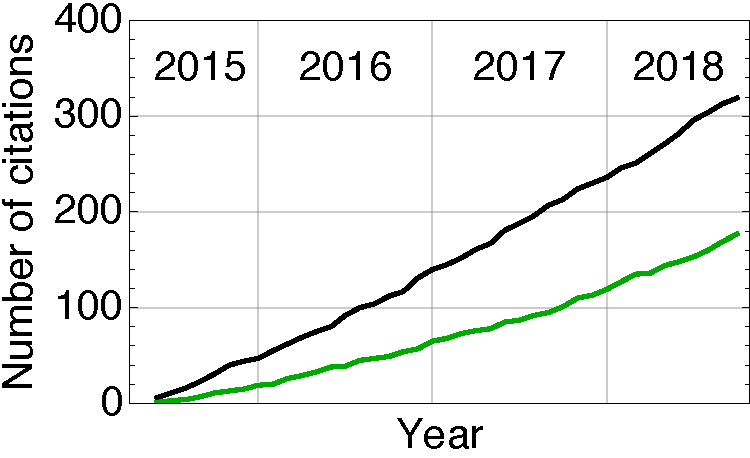
\includegraphics{figs/Introduction/citations_PP_TP.pdf}
    \caption{Citation history of the SHiP physics paper~\protect\cite{Alekhin:2015byh} (black) and of the SHiP Technical Proposal \protect\cite{Anelli:2015pba} since their initial publication in April 2015.}
    \label{fig:citations}
\end{figure}

While energy frontier is investigated at the LHC and drives the projects of the future colliders, the precision frontier is pursued at LHCb and elsewhere, the intensity frontier remains under-explored. It is the main goal of the SHiP experiment to make the break-through in this direction. In particular, the discovery potential of SHiP will allow to  explore the domain of  particle masses and couplings that are not accessible to the energy and precision frontier experiments and potentially find the particles that lead to neutrino masses and oscillations, explain  baryon asymmetry of the Universe and  shed the new light on the properties of dark matter (for a detailed discussion see \cite{Alekhin:2015byh}), even more so with the updated SHiP design described below.

SHiP experiment has received lots of attention from the particle physics community. The SHiP physics paper~\cite{Alekhin:2015byh} is a highly-cited document (see Fig.~\ref{fig:citations}),  many groups continue to explore the scientific potential of the experiment, making detailed predictions for models of feebly interacting particles.
Apart from the SHiP experiment, several dedicated intensity frontier experiments have been proposed in the recent years: CODEX-b~\cite{Gligorov:2017nwh},
MATHUSLA~\cite{Chou:2016lxi,Curtin:2017izq,Evans:2017lvd},
FASER~\cite{Feng:2017uoz,Feng:2017vli,Kling:2018wct}. Recognizing the importance of non-LHC physics, the CERN Management created in 2016 a dedicated Study Group “Physics Beyond Colliders” (PBC). 
Searches of heavy neutral leptons, dark photons, dark scalars and other super-weakly interacting light particles has been included in the scientific goals of many presently running experiments~\cite{Aaij:2014aba,Khachatryan:2015gha,Aad:2015xaa,Sirunyan:2018mtv,Izmaylov:2017lkv, Mermod:2017ceo,CortinaGil:2017mqf,Antusch:2017hhu,Drewes:2018gkc,Liventsev:2013zz,Kwon:2017anc,TheBelle:2015mwa,Lees:2017lec,Banerjee:2016tad,Aaboud:2018jbr,Aaij:2017rft}.



\subsection{Global concept of re-optimized experimental configuration}

\subsubsection{Muon shield}
Magnetized hadron stopper

\subsubsection{{Decay volume}}
Pyramidal frustum

\subsubsection{Detector layout}
Main changes to scattering spectrometer and decay spectrometer